\section{Introduction}
\label{mmf-sec:intro}

While even very early on, researchers realised, that cancers have different morphologies and clinical progression depending on the primary occurrence of the tumour (\autoref{intro-sec:cancer}), with the extensive sequencing of cancer specimen over the last decade, the mutational signatures of cancers came into focus. These signatures are specific and characteristic combinations of mutations, which stem from distinct biological processes. Among processes are exposure to DNA damaging agents like Chemotherapy treatment, tobacco and UV radiation, as well as biological intrinsic pathways errors in DNA-replication or -repair. As each of those processes has a more or less distinct profile of mutations \cite{Hollstein1991,Kucab2019} the analysis and deconvolution of the signatures involved in a patients mutational landscape can help diagnosing and treating a patient. While many signatures occur at a background level and are related to ``normal`` cellular processes like ageing \cite{Alexandrov2013}, others can point to defective mismatch repair or gain of function mutations in specific pathways, which then lead to new avenues of therapy for the patient \cite{Neil2017}.

Supplementary information and plots for this chapter are attached in the appendix and prepended with \ref{ch-mmfSuppMeth}.

\subsection{Mutational signature analysis}
\label{mmf-sec:signatureanalysis}
Traditionally the cancer mutational signature analysis entails a somatic variant calling process (\autoref{intro-sec:variantcalling}) followed by a counting and deconstructing step, which assigns weights to the individual signatures. These signatures are precompiled list of mutation count relations (\autoref{fig:sig7a}). While the individual SNP already contains valuable information, there is an improvement in granularity when also counting the base up and downstream of the change. This expands the feature space of counts from the six base classes of SNPs (C>A, C>T, C>G, T>C, T>A, and T>G) to 96 unique trinucleotide contexts \cite{Alexandrov2013}. While there technically are six more base changes and several  more trinucleotide contexts combinatorially possible, they can be collapsed into the afore mentioned 96 by using the reverse complement of the change.

\begin{figure}[!ht]
\centering
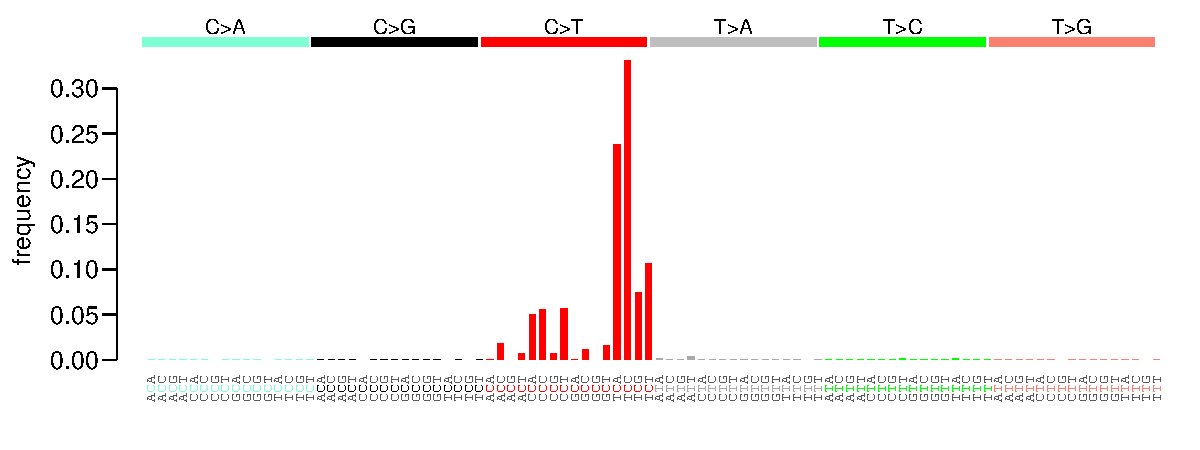
\includegraphics[width=.99\linewidth]{Figures/MisMatchFinder/SBS7aSignature.pdf}
\caption[Trinculeotide count contributions for single base substitution (SBS) signature 7a]{Trinculeotide count contributions for SBS signature 7a (UV exposure); values taken from \protect\textcite{Alexandrov2020}}\label{fig:sig7a}
\end{figure}

Additionally to the single base substitution (SBS) there now exist doublet base substitution signatures and InDel signatures for somatic mutations of cancers \cite{Alexandrov2020}, which are all based on the same principle and enable a higher precision for stratification of similar cancer subtypes and DNA damaging agents.

\subsection{Restrictions and pitfalls of standard signature analysis}
Especially for cancer samples, the focus usually is on somatic variants of the sample. This requires a fairly deep sequencing of the tumour sample with at least WES or WGS and for optimal results, a germline sample for tumour-normal variant calling is required as well to not have noise from potentially retained germline variants (\autoref{intro-sec:somaticcalling}). This means the cost of the data of the analysis is surprisingly high for a fairly diffuse result of signatures that contribute to the variants found. This is especially relevant when it comes to clinical diagnostic tools, where every biopsy of the patient is valuable and a germline sample might not always be available. For an analysis, which is based on the averaged and aggregated somatic variants to require a high quality input could be seen as counter-intuitive. Especially, as the analysis will always report signatures, even if there are virtually no variants reported, it will still suggest a mixture of potentially clinically relevant signatures, even if the patient is healthy.

\subsection{Overview}
 This chapter describes a newly developed method, which allows the detection of somatic signatures from low coverage WGS of cfDNA. This method potentially enables the non-invasive monitoring of patients and possibly screening of at-risk individuals with very little cost, instead of the cost intensive current methods.
